\documentclass[sigconf]{acmart}

\graphicspath{ 
	{./figures/}
	%  Animations of some figures (exported as PNG) are locaten in subdirectories.
	%  For example:
	%    figures/Average/Curves/"
	%    figures/OutsidePoints/png/"
	%  Figures I took from others are in subdirectories whos names start with
	%  "By" followed by the Authors name
	%    figures/ByCiccone/
}

% https://tex.stackexchange.com/a/346309/62013
\settopmatter{printacmref=false} % Removes citation information below abstract
\renewcommand\footnotetextcopyrightpermission[1]{} % removes footnote with conference information in first column
%\pagestyle{plain} % removes running headers

\usepackage{booktabs} % For formal tables

\acmConference{Computational Photography Project}{June 2019}{Bonn}

% Use the "authoryear" citation style, and make sure citations are in [square brackets].
\citestyle{acmauthoryear}
%\citestyle{acmnumeric}
\setcitestyle{square}

% A useful command for controlling the number of authors per row.
% The default value of "authorsperrow" is 2.
%\settopmatter{authorsperrow=4}
%   Had to comment out this line since it prevented the PDF from building.

% % % % % % % % % % % % % % % % % % % % % % % % % % % % % % % % % % % % % 
%  Add packages to your TexLive instllation:
% % % % % % % % % % % % % % % % % % % % % % % % % % % % % % % % % % % % % 
% To build this document you need to have a few LaTeX packages installed.
% In TexLive You can install packages like "mathtools" from CTAN using
% the "TexLive Package Manager":
%   tlmgr install mathtools

% % % % % % % % % % % % % % % % % % % % % % % % % % % % % % % % % % % % % 
%  CUSTOM COMMANDS:
% % % % % % % % % % % % % % % % % % % % % % % % % % % % % % % % % % % % % 

% % % % % % % % % % % % % % % % % % % % % % % % % % % % % % % % % % % % % 
% Row Vector:
% https://tex.stackexchange.com/a/266741/62013
% % % % % % % % % % % % % % % % % % % % % % % % % % % % % % % % % % % % % 

\newcommand{\vect}[1]{\begin{bmatrix} #1 \end{bmatrix}}
\newcommand{\mat}[1]{\begin{bmatrix} #1 \end{bmatrix}}

% % % % % % % % % % % % % % % % % % % % % % % % % % % % % % % % % % % % % 
% Make vector bold instead of arrow
% https://tex.stackexchange.com/a/327896/62013
% % % % % % % % % % % % % % % % % % % % % % % % % % % % % % % % % % % % % 
\let\vec\mathbf

% % % % % % % % % % % % % % % % % % % % % % % % % % % % % % % % % % % % % 
% Absolute Value and Norm Symbols
% https://tex.stackexchange.com/a/43009/62013
% % % % % % % % % % % % % % % % % % % % % % % % % % % % % % % % % % % % %
\usepackage{mathtools}
% provides: \coloneqq, \eqqcolon, 
\DeclarePairedDelimiter\abs{\lvert}{\rvert}%
\DeclarePairedDelimiter\norm{\lVert}{\rVert}%
\DeclarePairedDelimiter{\ceil}{\lceil}{\rceil}% https://tex.stackexchange.com/a/42274/62013 
% Swap the definition of \abs* and \norm*, so that \abs
% and \norm resizes the size of the brackets, and the 
% starred version does not.
\makeatletter
\let\oldabs\abs
\def\abs{\@ifstar{\oldabs}{\oldabs*}}
%
\let\oldnorm\norm
\def\norm{\@ifstar{\oldnorm}{\oldnorm*}}
\makeatother
%
%Example:
%\newcommand*{\Value}{\frac{1}{2}x^2}
%\begin{document}
%	\[\abs{\Value}  \quad \norm{\Value}  \qquad\text{non-starred}  \]
%	\[\abs*{\Value} \quad \norm*{\Value} \qquad\text{starred}\qquad\]
%\end{document}

% % % %
% Convenience Macros
% https://en.wikibooks.org/wiki/LaTeX/Macros#New_commands
% % % %

% Abbreviation for the norm of a vector using the suffix package
% to define the corresponding starred version:
%   https://tex.stackexchange.com/a/4388/62013
\usepackage{suffix}
\newcommand\vn[1] {\norm{\vec{#1}}} % vector norm
\WithSuffix\newcommand\vn*[1]{\norm*{\vec{#1}}} % vector norm

% % % % % % % % % % % % % % % % % % % % % % % % % % % % % % % % % % % % % 
% Less Space between equations and text
% https://latex.org/forum/viewtopic.php?f=47&t=15371#p56484
% % % % % % % % % % % % % % % % % % % % % % % % % % % % % % % % % % % % %
\makeatletter
\g@addto@macro{\normalsize}{%
	\setlength{\abovedisplayskip}{0pt}
	\setlength{\abovedisplayshortskip}{0pt}
	\setlength{\belowdisplayskip}{0pt}
	\setlength{\belowdisplayshortskip}{0pt}}
\makeatother

% % % % %
% Physics package for derivative commands:
% https://tex.stackexchange.com/a/225527/62013
\usepackage{physics}
% Example
% Rewrite this:
%	\[
%   E_C(c)= \norm{\frac
%		{\partial^2 c(s)}
%		{\partial s^2}	
%	}^2
%	\]
% as this:
%	\[
%   E_C(c)= \norm{
%		\pdv[2]{c(s)}{s}	
%	}^2
%	\]

% % % % % %
\usepackage{subfig}
% Plot two figures side by side:
% https://tex.stackexchange.com/a/37583/62013

% % % % % %
\usepackage{dsfont}
% https://tex.stackexchange.com/a/26640/62013
% Adds nice fonts. For example for the "indicator function":
% \[ \mathds{1} \]

% % % % % %
% Set graphics pathes:
%\graphicspath{ {figures/taken} }

% % % % % % % % % % % % % % % % % % % % % % % % % % % % % % % % % % % % % 
% end of preamble.
% % % % % % % % % % % % % % % % % % % % % % % % % % % % % % % % % % % % % 

\begin{document}

% Title. 
% If your title is long, consider \title[short title]{full title} - "short title" will be used for running heads.
\title{Project Report: Learning Polarization Difference Imaging}
%\title[Flow Curves]{An Intuitive Interface for Coherent Scene Deformation}

% Authors.
\author{s6biulus}
\affiliation{%
  \department{Department of Computer Science}
  \institution{University of Bonn}}
\email{s6biulus@uni-bonn.de}

\author{Tim Oliver Sauermann}
\affiliation{%
  \department{Department of Computer Science}
  \institution{University of Bonn}}
\email{tim.sauermann@sauermannonline.de}

\author{Daniel Hubert Biskup}
\affiliation{%
  \department{Department of Computer Science}
  \institution{University of Bonn}}
\email{daniel@biskup.email}

%keywords
%\keywords{not ray tracing, not global illumination, not octrees, not quadtrees}

% A "teaser" figure, centered below the title and authors and above the body of the work.
\begin{teaserfigure}
  \centering
  \includegraphics[width=6.0in]{figures/teaser.png}
  \caption{Polarization images captured by our setup (center), their sum (left) and the result of subtracting one form the other (right)}
  \label{fig:teaser}
\end{teaserfigure}

% Processes all of the front-end information and starts the body of the work.
\maketitle

\section{Motivation}
For some tasks it is required to get images that separate the direct and indirect reflected components of a light source illuminating a scene. This can be achieved by the technique of polarization difference imaging \cite{PDI}. Since this is a quiet time-consuming process that requires special hardware a more simple and effective way to get an image separated into this two components would be desirable. This project tries to realize that using deep learning mechanisms on normal pictures of human faces.

\section{Image Acquisition}
Any project involving Deep Learning requires training data. To this end we devised a setup (see figure~\ref{fig:personDay} and \ref{fig:personNight}) which allows us to capture pairs of polarized images of human faces. An example of an image pair captured this way can be seen in figure~\ref{fig:teaser}.

Using duct tape, opaque black curtains were attached to the lab rooms windows as to ensure a consistently dark environment.

To capture a pair of polarization images, we take two images of the same static scene. For each pair, one image each is taken while the scene is illuminated with horizontally and vertically polarized light respectively. As a camera we use the \emph{Flir Grasshopper 3} with a linear polarizing film in front of its lens (see figure~\ref{fig:setupWithFilter}).

Polarized light gets unpolarized when it's indirectly reflected from the subject, e.g. due to sub surface scattering in the human skin. In the case of direct reflection it keeps it's original polarization. Thus, when the filter in front of the camera absorbs all horizontally polarized light and we take an image of the scene under horizontally polarized illumination ( i.e. the polarization of the light source and the camera are parallel to each other) the camera will receive the full amount of directly reflected light but just the parallel components of the unpolarized light (see figure~\ref{fig:teaser} top).
On the other hand, when the scene is illuminated with with vertically polarized light (i.e. light and filter are cross polarized to each other) no directly reflected light (i.e vertically polarized light ) will pass the horizontal polarization filter in front of the camera, while the unpolarized (i.e. not directly reflected light) will (see figure~\ref{fig:teaser} bottom).

This fact can be exploited by subtracting the cross polarized image from the parallel polarized image which yields an image that contains only the directly reflected light (see figure~\ref{fig:teaser} right). Adding the cross polarized image and the parallel polarized image up yields an naturally looking image (see figure~\ref{fig:teaser} left).

To be able to alternate between horizontally and vertically polarized illumination of the scene, we use two identical LED-chips of type \emph{Samsung LH351B-RT}, attached to a star-board for cooling and connect them to a computer via an \emph{Arduino Nano} which is controlling a simple mosfet-driver and in that way enables us to control them using a Python script. We favoured a simple driver like this over a dedicated constant-current driver to enable us to use high switching speeds. The LEDs are mounted on lenses collimating the beams to an angle of $8^\circ$ and attached to a polarizing beamsplitter cube of type \emph{ThorLabs CCM1-PBS251} using custom 3D printed mounting brackets and duct tape (see figure~\ref{fig:setupWithoutFilter}).

\begin{figure}
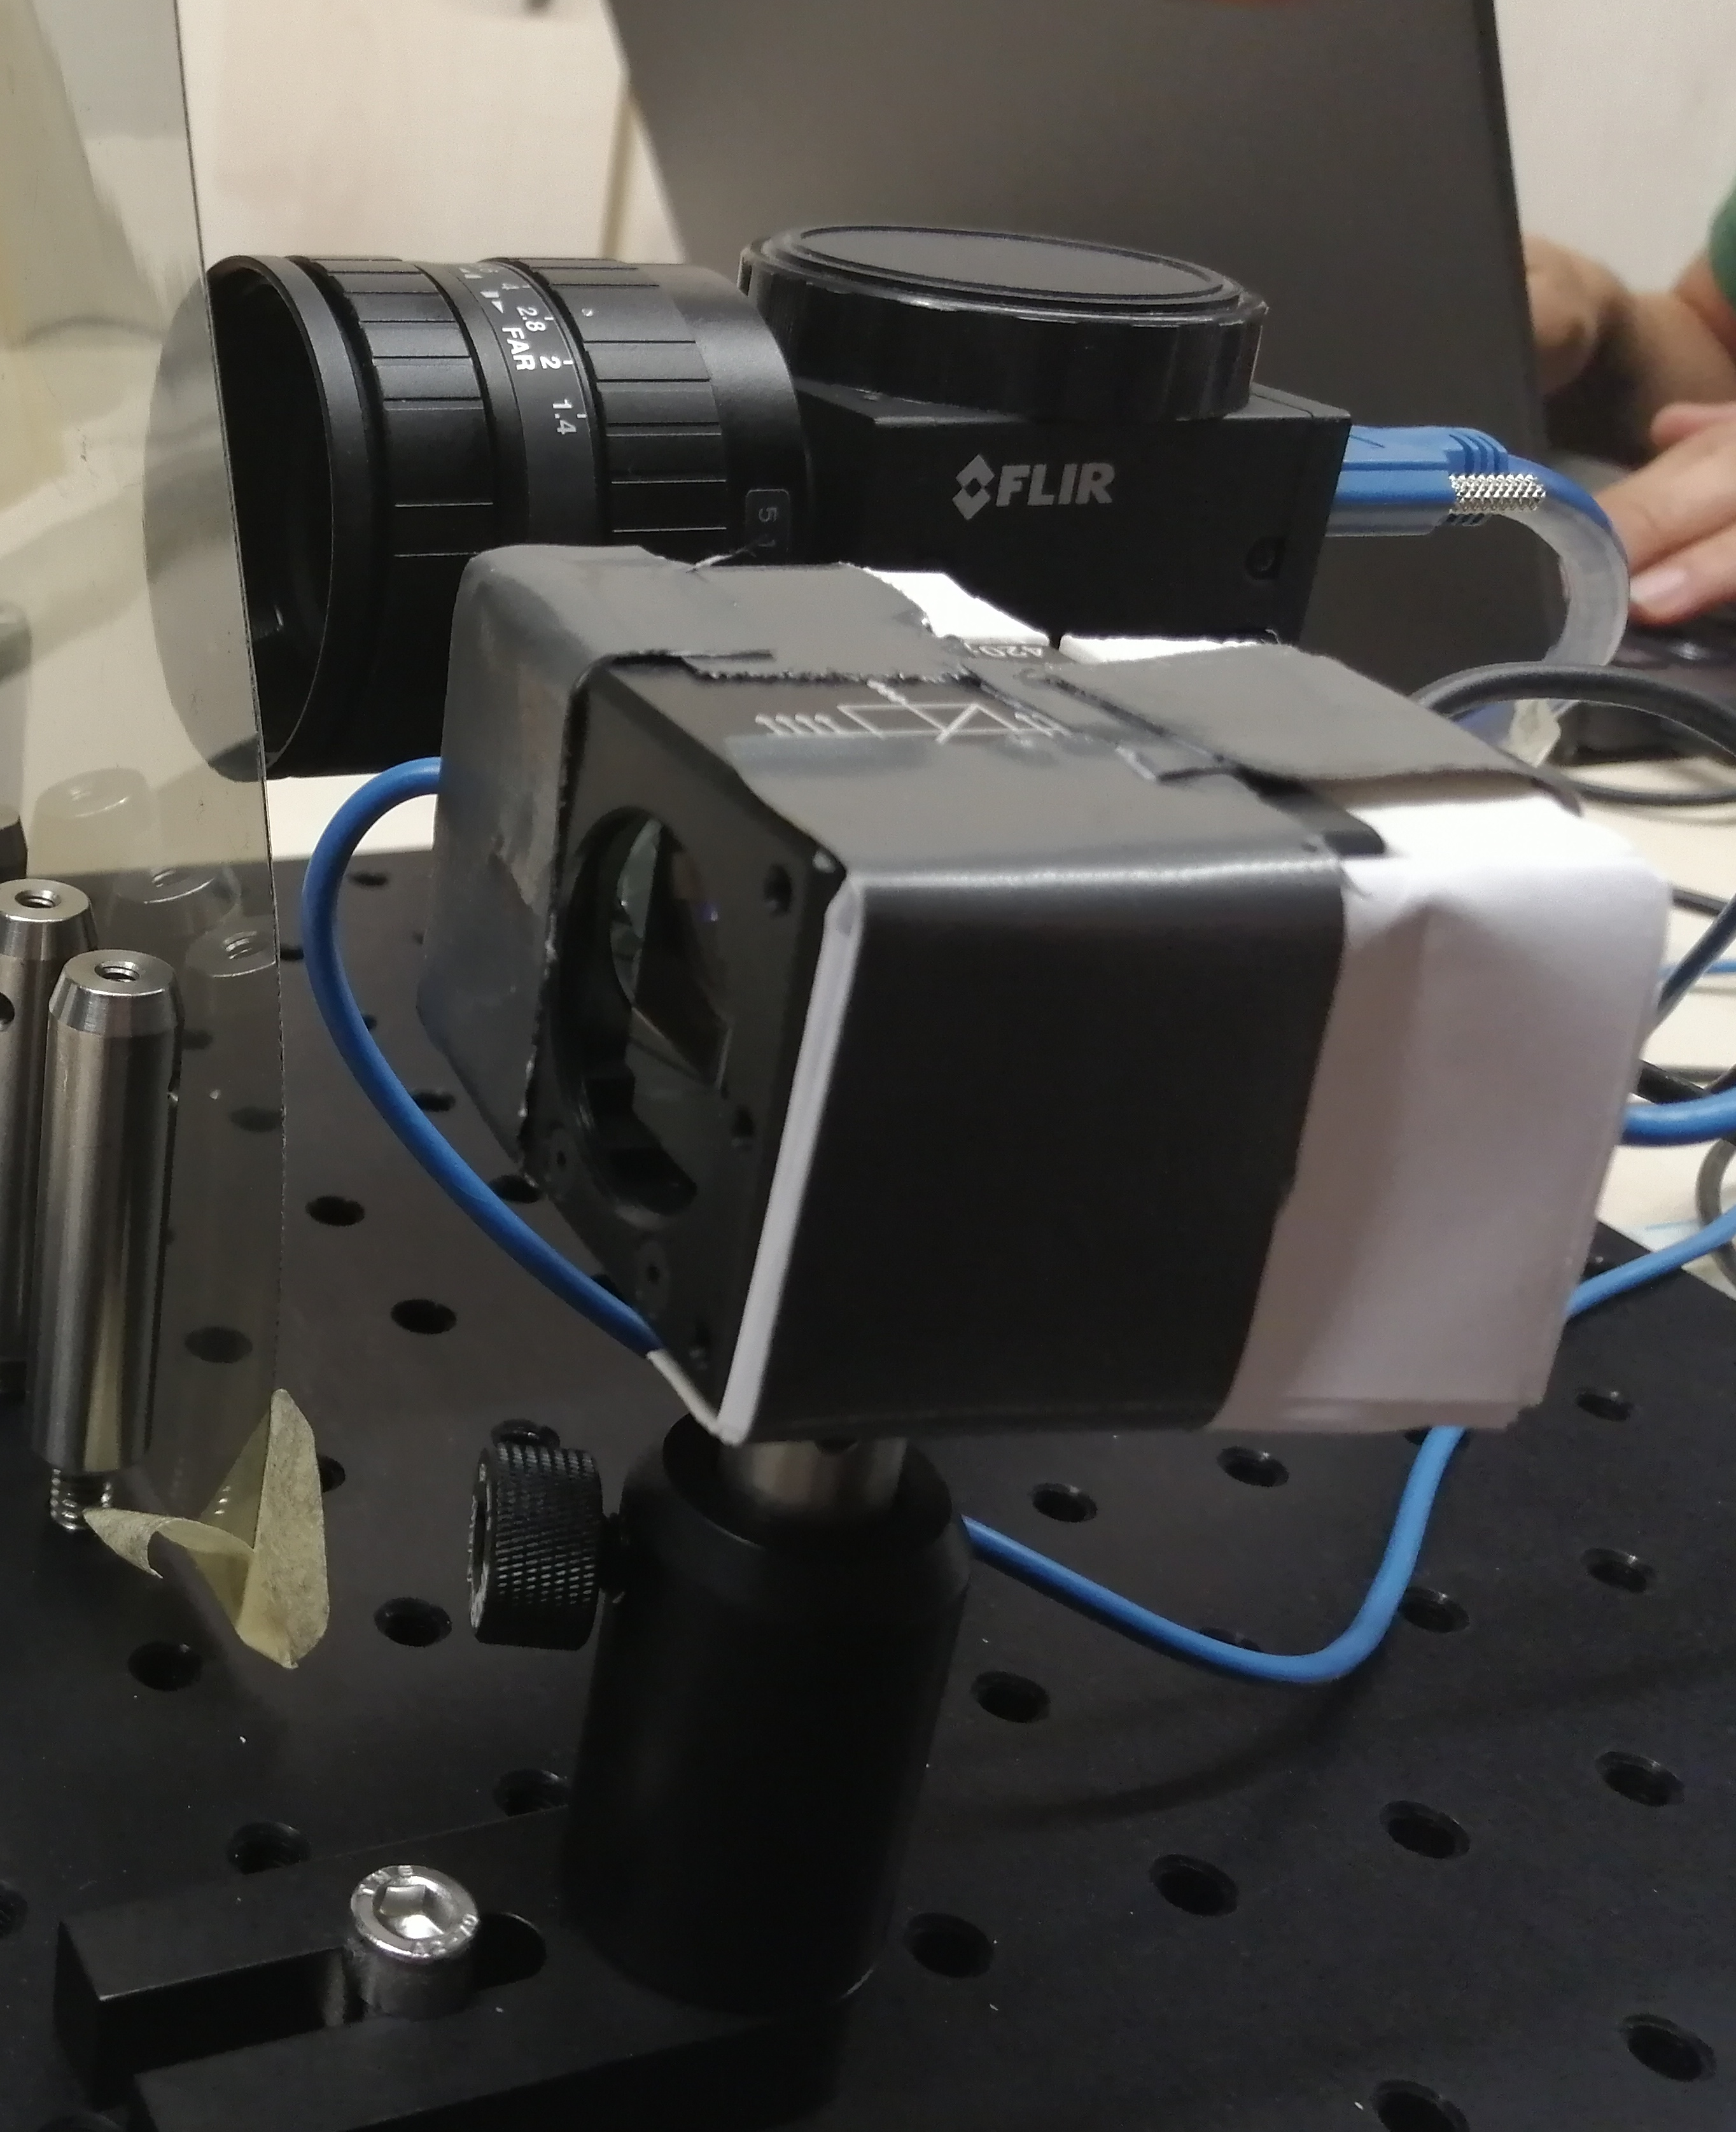
\includegraphics[width=0.9\linewidth]{figures/withFilter2cropped.png} 
\caption{Camera with polarizing filter and LEDs attatched to polarizing beamsplitter cube}
\label{fig:setupWithFilter}
\end{figure}

\begin{figure}
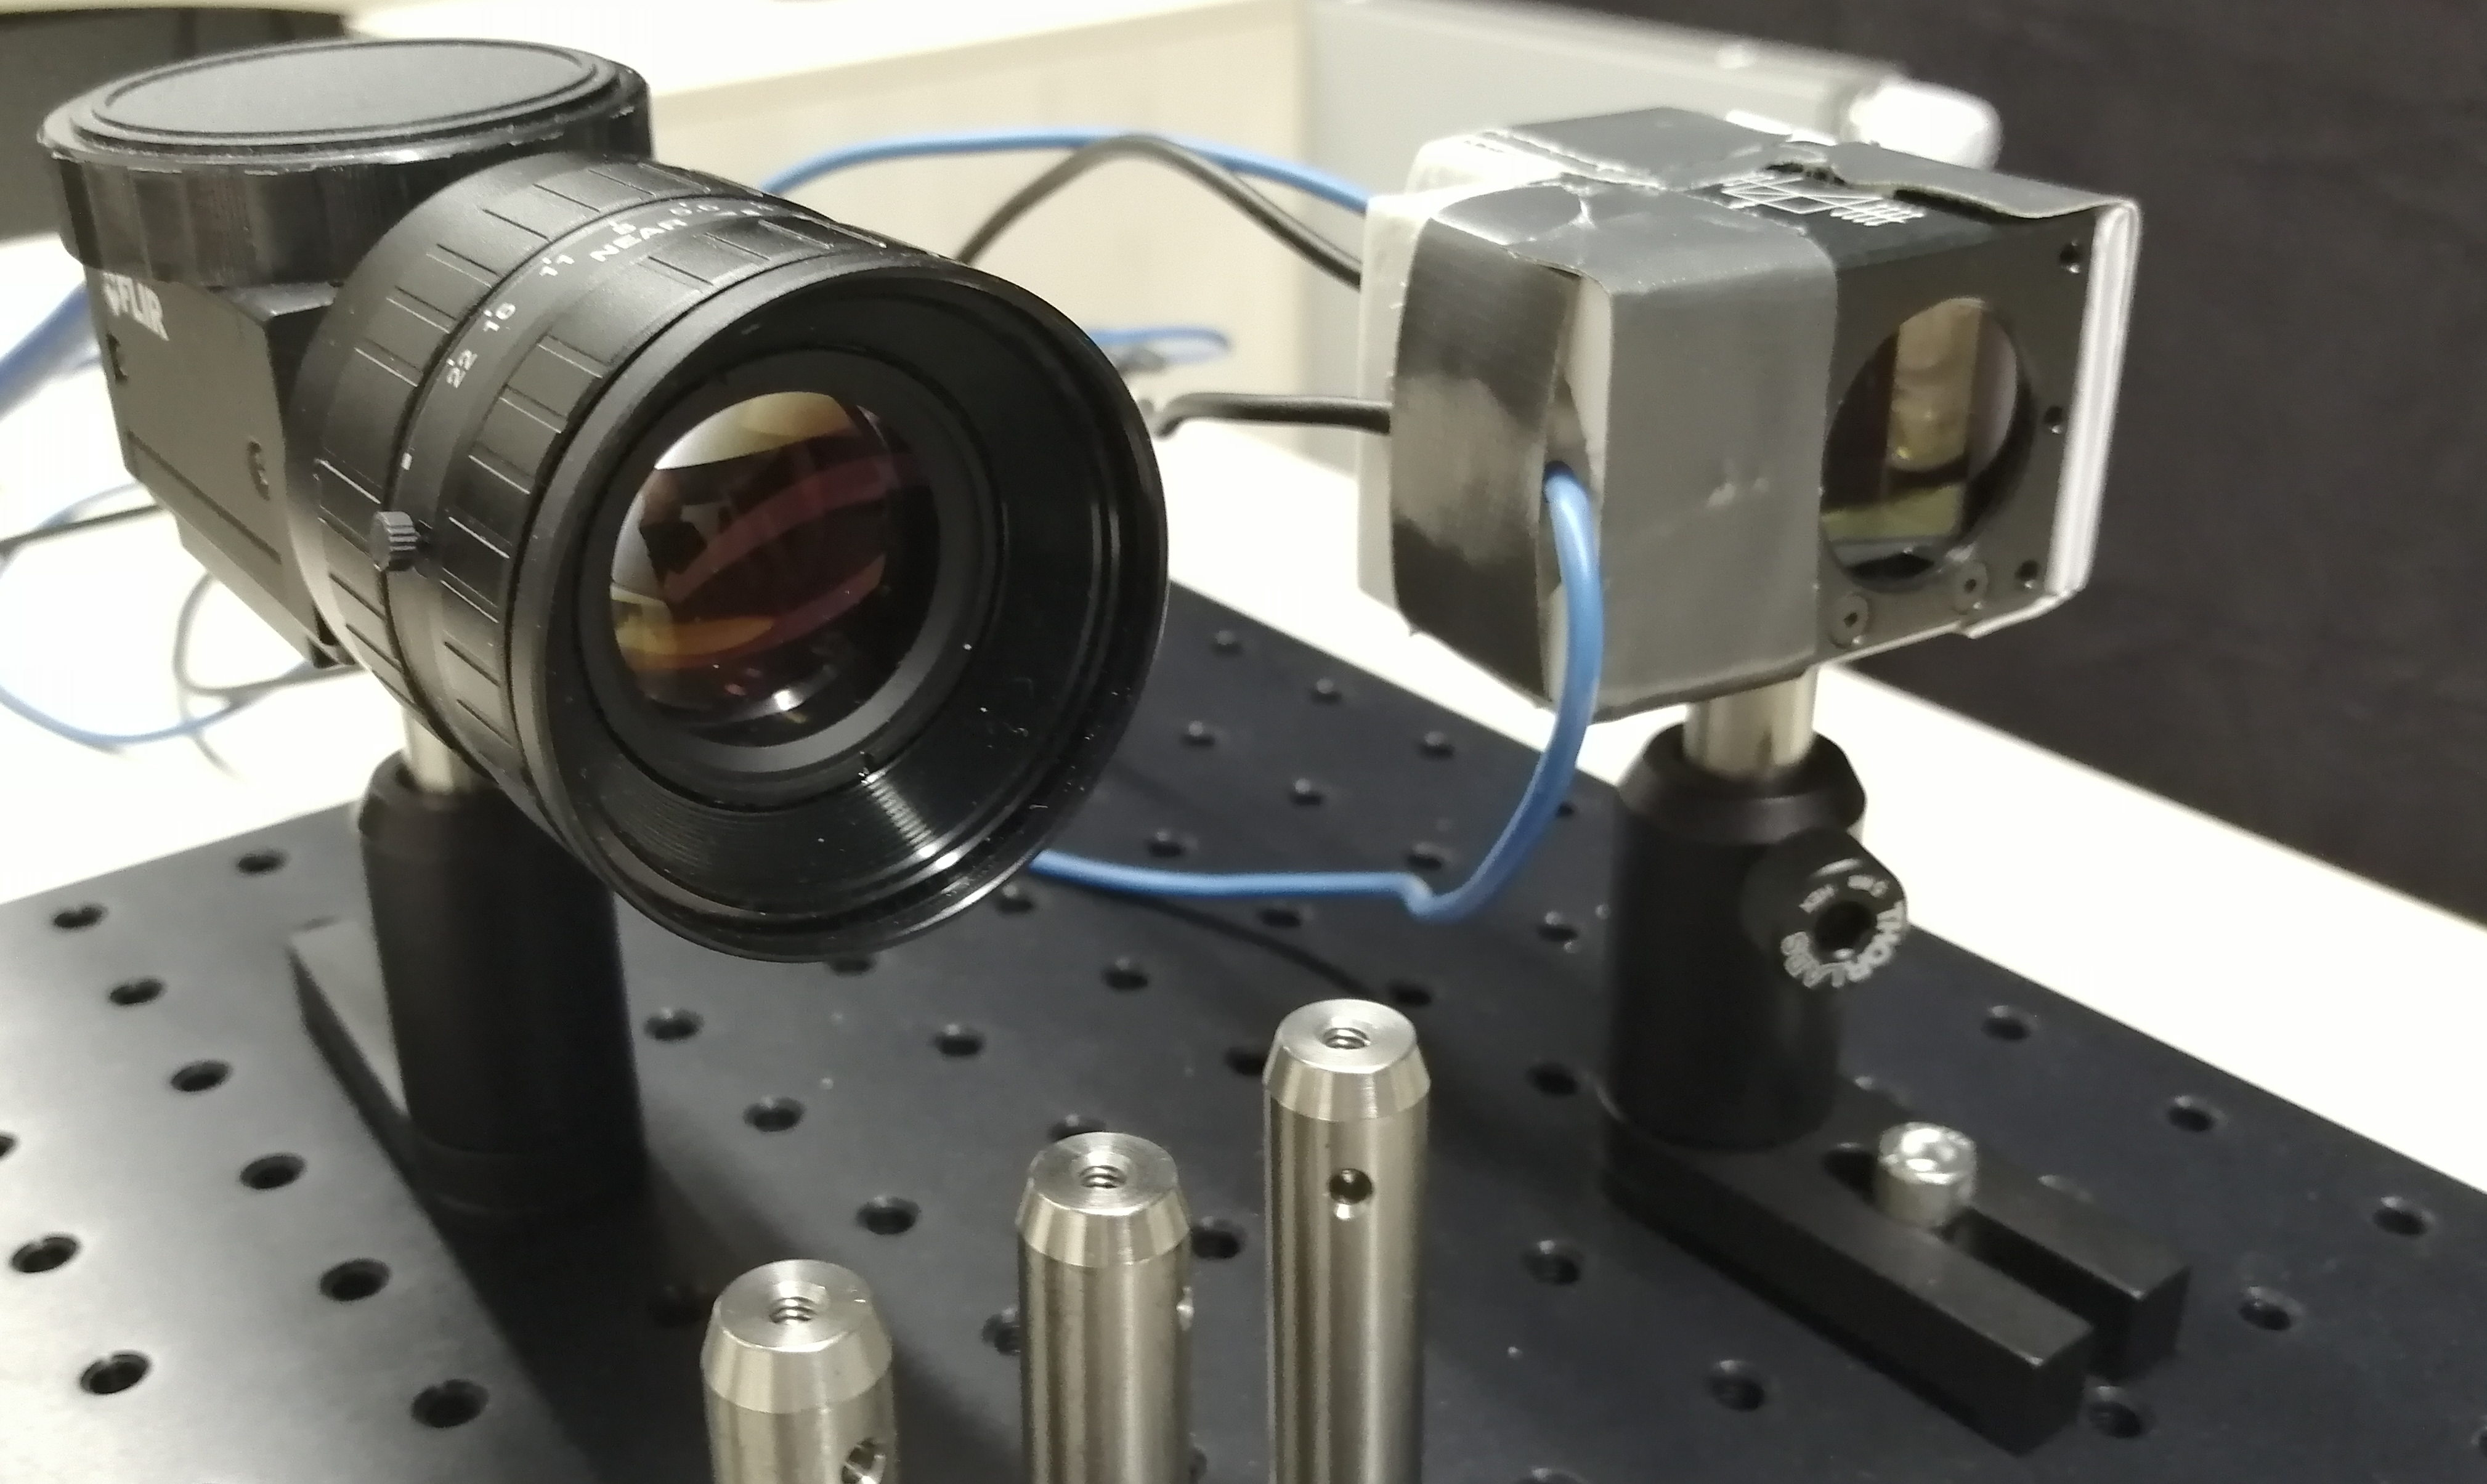
\includegraphics[width=0.9\linewidth]{figures/CamAndLEDcropped.png} 
\caption{Camera and light source}
\label{fig:setupWithoutFilter}
\end{figure}

\begin{figure}
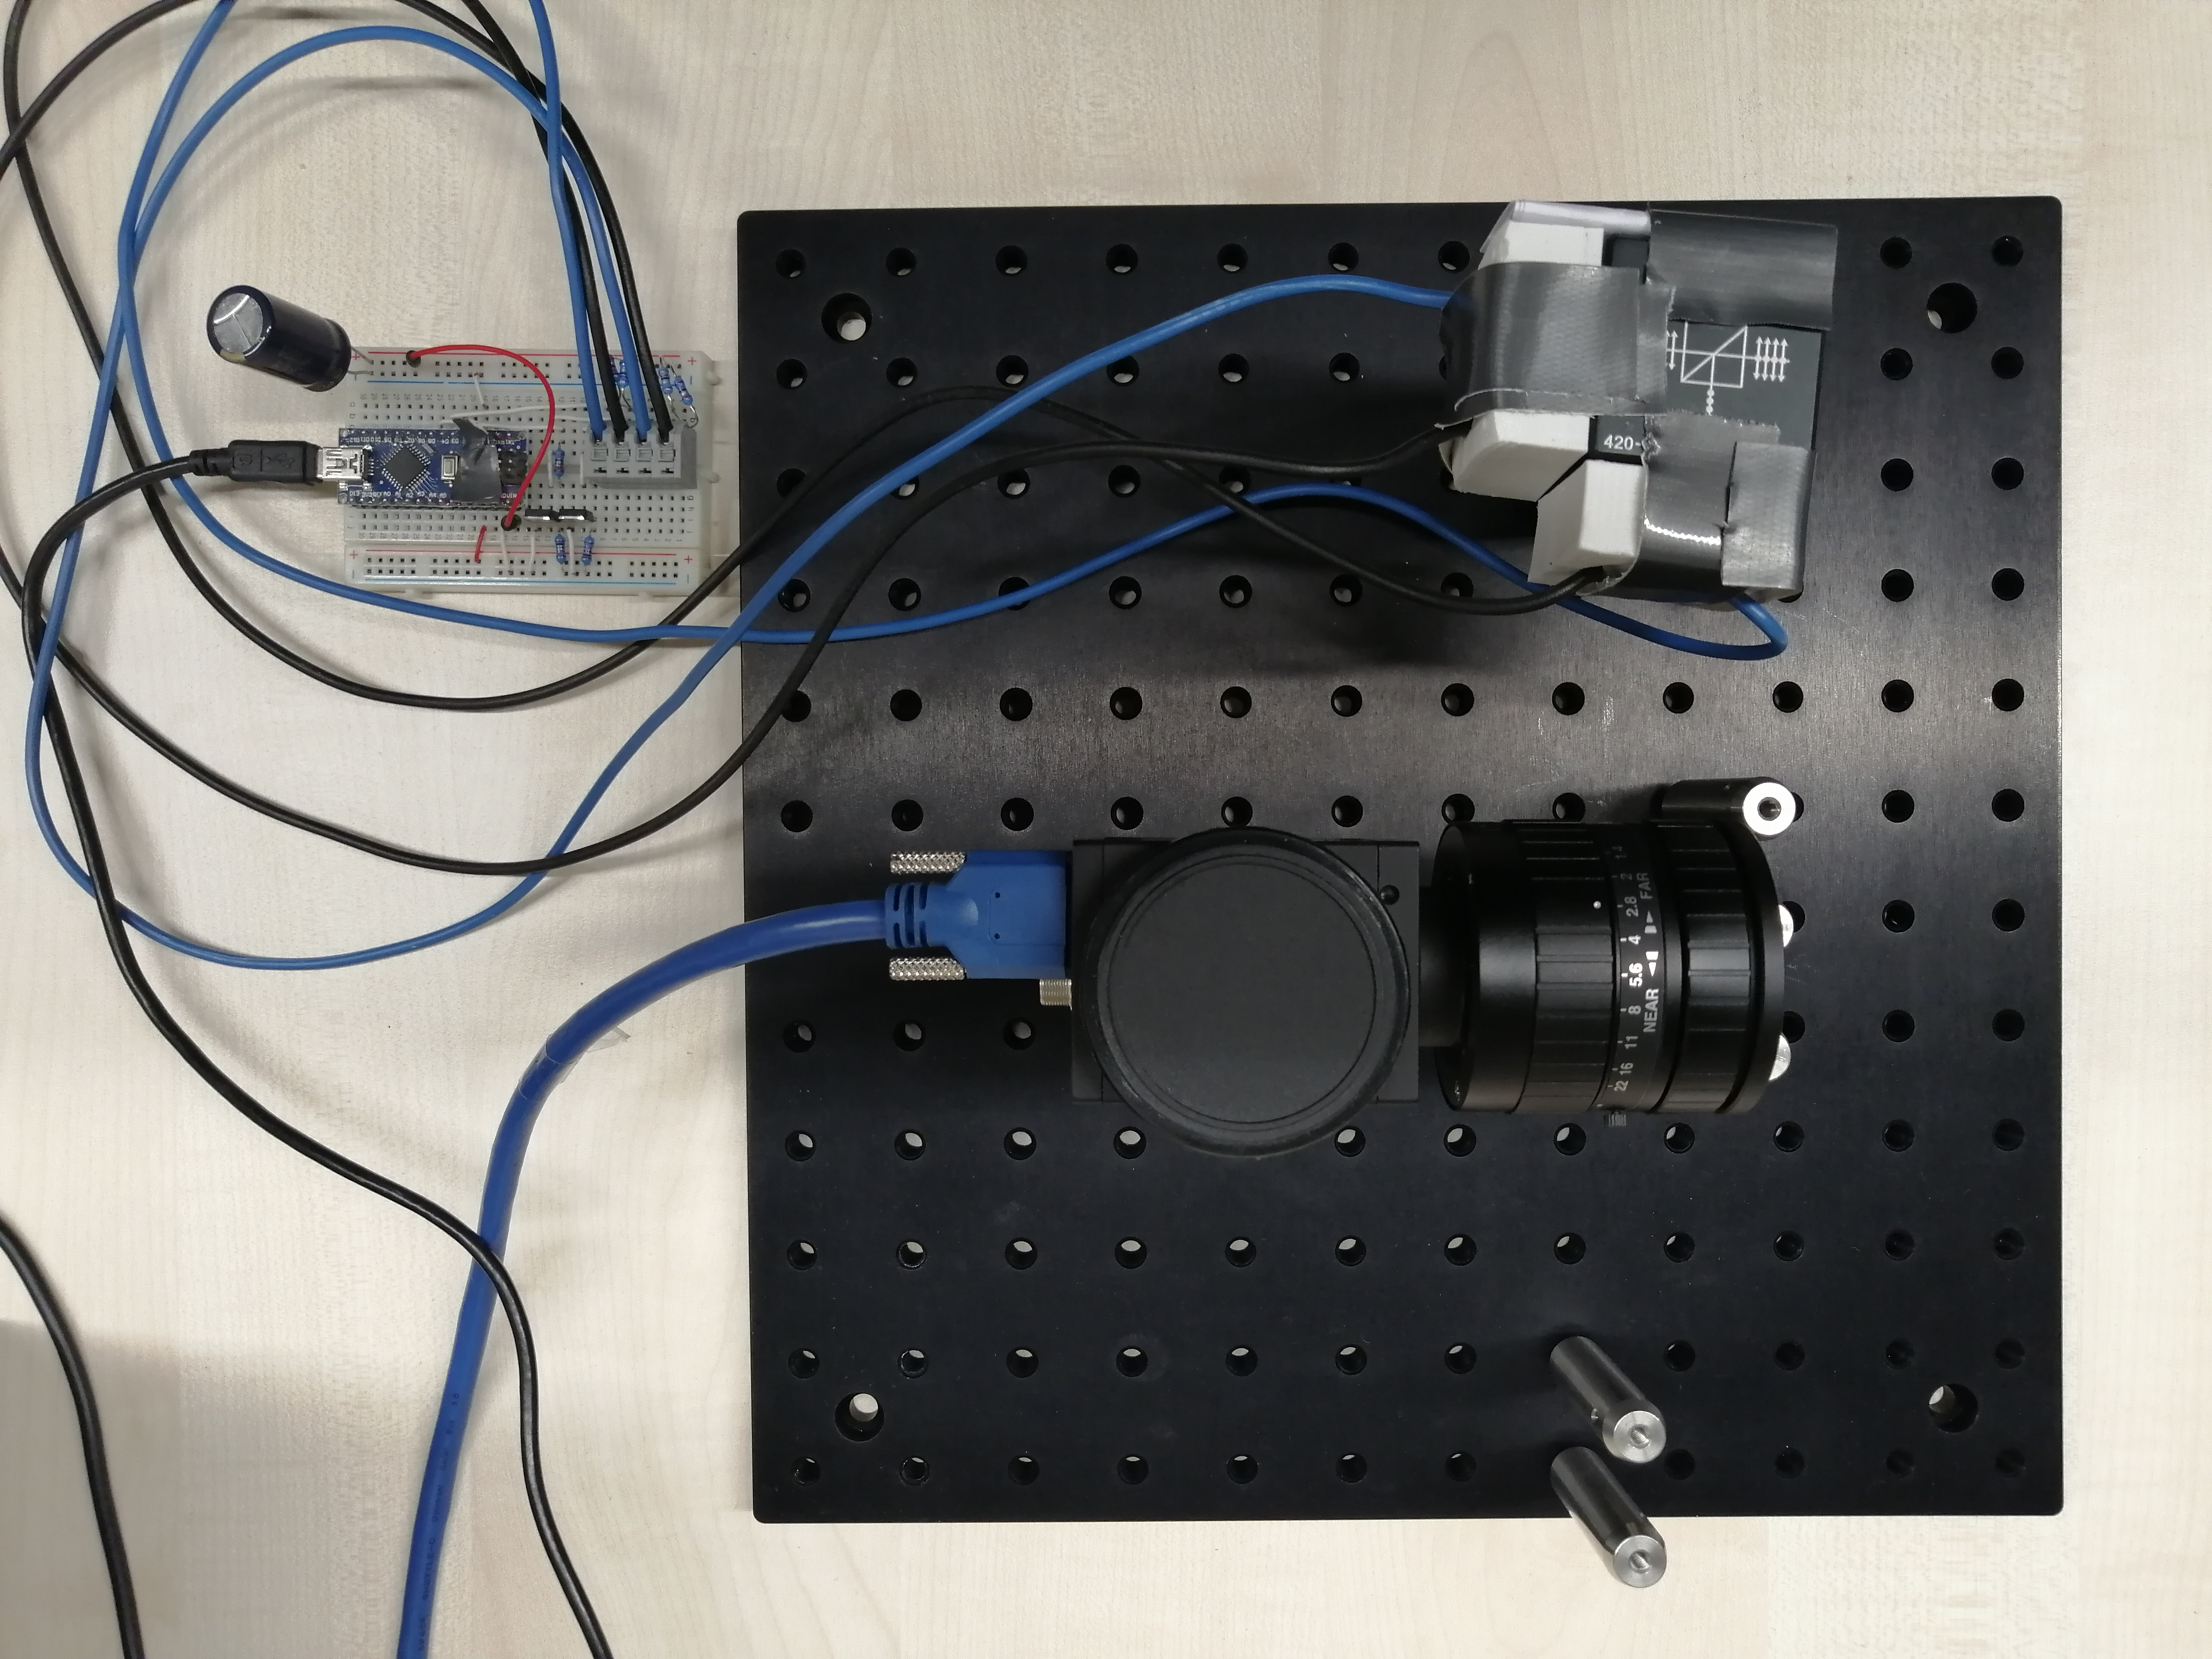
\includegraphics[width=0.9\linewidth]{figures/setupTop.jpg} 
\caption{Setup from above. The Arduino to control the LEDs can be seen on the left.}
\label{fig:setupTop}
\end{figure}

\begin{figure}
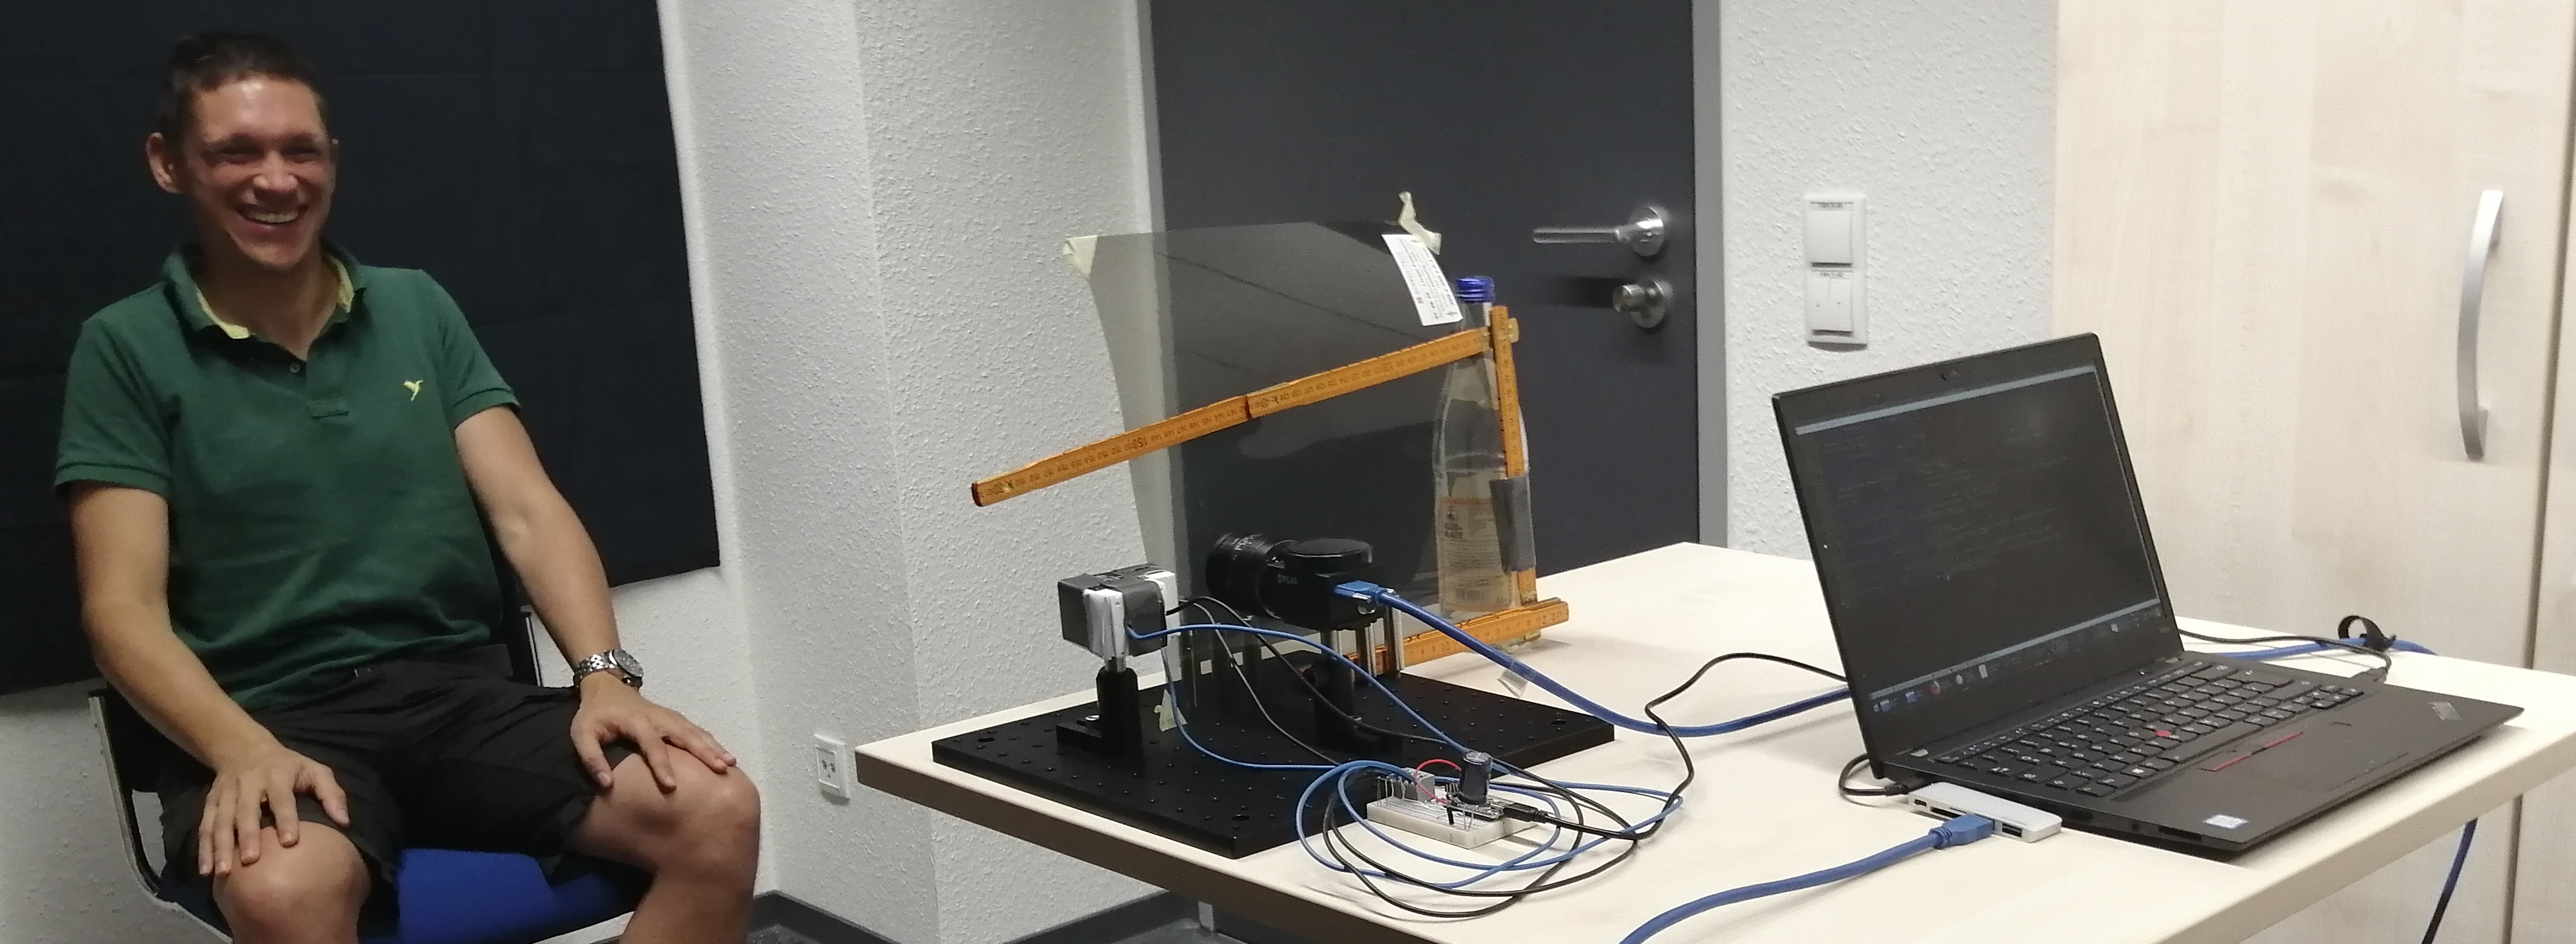
\includegraphics[width=0.9\linewidth]{figures/personCropped.png} 
\caption{Image acquisition setup}
\label{fig:personDay}
\end{figure}

\begin{figure}
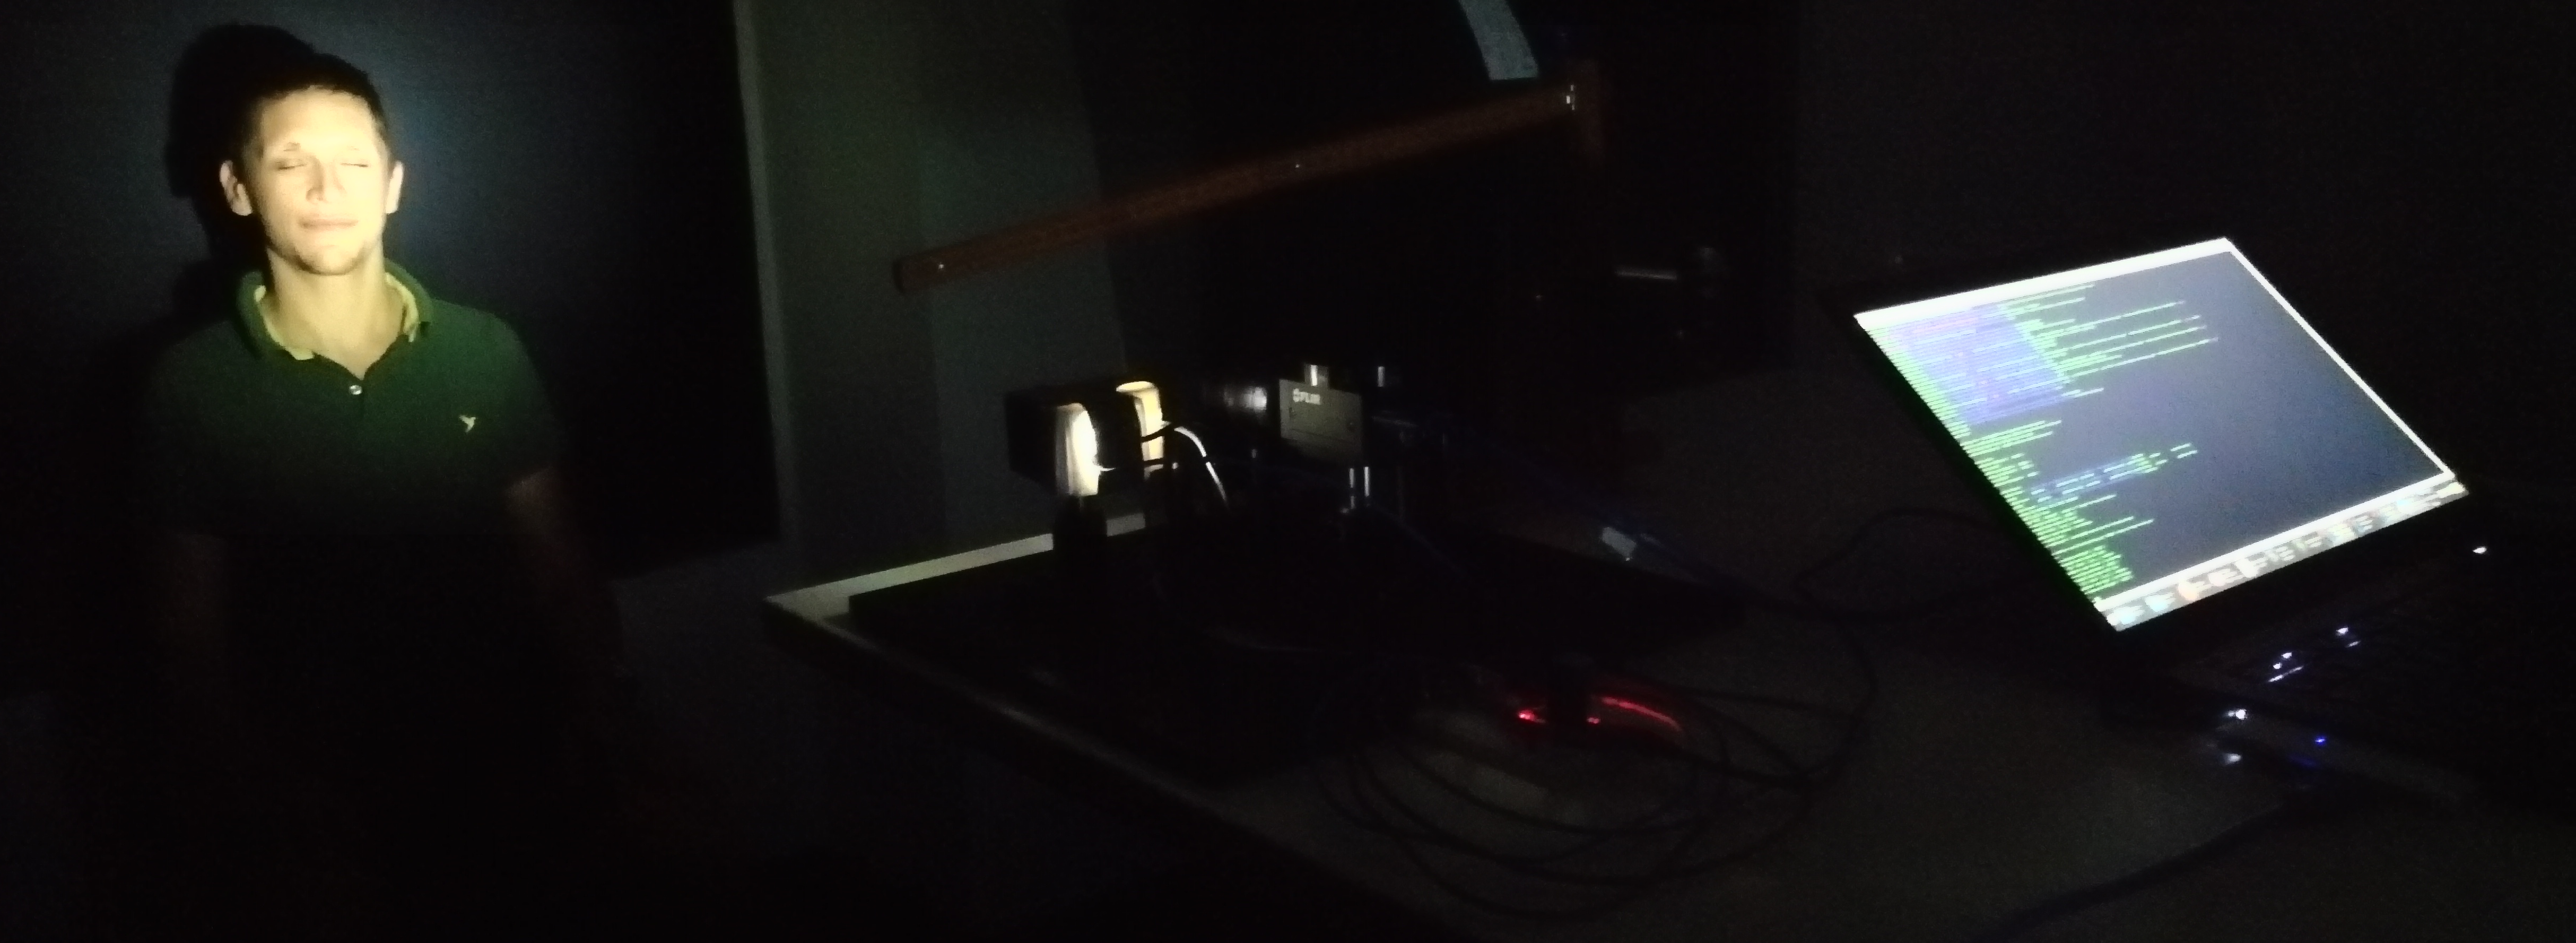
\includegraphics[width=0.9\linewidth]{figures/personNightCropped.png} 
\caption{Image acquisition setup (in use)}
\label{fig:personNight}
\end{figure}

To ensure, that two images of the same pair are aligned to each other as good as possible the subject is not allowed to move (e.g. change it's facial expression) in between the two shots belonging to the same pair of polarization images. To minimize the risk the two images are taken rapidly after another using the internal buffer of the camera. To still allow for a reasonably fast acquisition images of different facial expressions or directions we give the subject about one second of time to move between taking image pairs, this time is also used to transfer the pictures from the camera to the PC and save them to disk. This allows for an effective acquisition rate of about 3600 polarization image pairs an hour.

An alternative way to using two polarized LEDs and a single camera with a polarization filter in front of it's lens would have been to use one polarized LED and two cameras, both attached to the polarizing-beamsplitter cube. This would have allowed us to capture a huge data set faster, since both cameras can be triggered simultaneously (by having one software triggered camera hardware triggering the other) which remedies the problem of miss-alignment between two images of the same pair due to movement of the captured subject. Then the subject could just slowly move its head while the cameras produce multiple images per second. In contrast, the image acquisition rate of our setup is much slower.
Even though this method of acquisition is potentially faster then ours we decided against it since using two cameras comes with its own set of technically intricate challenges. Most noteworthy, the two cameras have to be perfectly aligned to each other. This is very hard to archive and worthy of a project on its own. Furthermore a continually moving object would introduce motion blur into the images, potentially requiring the use of de-blurring techniques which would make the pre-computations even more complex. This problem gets even more noticeable since the power of the required point-light-source can't exceed a certain limit without the risk of taking severe damage to the subjects eyes. 

Following is a list of the technical equipment used:
\begin{itemize}
  \item Camera: \emph{Flir Grasshopper 3, model: GS3-U3-23S6C-C}
  \item Two LEDs: \emph{Samsung LH351B-RT Chips 5000K @ ~1200mA 3,1V ~3,8W}
  \item LED controller: \emph{Arduino Nano}
  \item Broadband Polarizing Beamsplitter Cube: \emph{ThorLabs CCM1-PBS251/M}
  \item Linear polarizing film: \emph{Screen-tech ST-38-20 - Linear Polarisator}
  \item Duct Tape: \emph{Ferociously Strong T-Rex Duct Tape}
\end{itemize}

\section{Learning}
The goal of the learning part of this project is to train a network which outputs either a parallel polarized image or a crossed polarized image from a given input image. This problem is very similar to Image-Denoising in a sense that one of the polarized images could be thought of as noise and that way could be removed from the input image, so that the other polarized image remains. This way both polarized images are accessible. In order to solve this problem, we combined ResNet- and Auto-Encoder-architectures.

We used an auto-encoder-architecture, which is a neural network architecture, that combines convolution and deconvolution layers. The convolution layers with 2 strides downsample the image in every layer, whereas the deconvolution layers with 2 strides upsample the image. While the convolution layers act like feature extractors, the deconvolution layers recover the details of the image content. Unlike segmentation problems, we did not use Max Pooling between layers in order to downsample, since recovering minor details of the image is very important in the given context. Generally deeper networks produce better results, since the network can express more complex non-linearities as the layers increase. In conclusion we wanted to use a very deep network for solving this problem, which is opposed by the problem that deep networks suffer from the problem of vanishing gradients. Skip connections, or residuals, in a ResNet architecture can solve this problem to some extend. The skip connections in ResNet feed the activation unit of a layer directly to a deeper layer of the network. With the addition of the skip connections connecting every two convolutional layers to their corresponding, mirrored deconvolutional layers, our network will be less affected by the vanishing gradient problem (see Figure~\ref{fig:NetworkArchitecture}).

\begin{figure}[h]
	\centering
	\includegraphics[width=\linewidth]{figures/network.png}
	\caption{The architecture of the network}
	\label{fig:NetworkArchitecture}
\end{figure}

Since the data collection process takes a long time for our problem, we created a mock-dataset to create an initial network and train it. The idea is to create a mock-dataset which consists of compositions of an orange image with black background and an cat image, so that these could be used to train the initial network (see Figure~\ref{fig:CatsAndOranges}). Since the operation to separate this overlaid images is equivalent to the operation we are planning to do with our actual problem, then we can use the same network for our original problem after verifying that it is possible to train the network successfully. Only slight by changes of its parameters would be necessary. The mock-dataset consists of 12,500 cat-images, composed with orange-images. The cat images were obtained from the "Dogs vs. Cats"-dataset from https://kaggle.com.

\begin{figure}[h]
	\centering
	\includegraphics[width=\linewidth]{figures/kitties.png}
	\caption{The mock dataset}
	\label{fig:CatsAndOranges}
\end{figure} 

%\section{[DEV ONLY] Testing some citations....}
%\cite{rain} \\
%\cite{ResNet} \\
%\cite{VeryDeepCNN} \\
%\cite{ConvolutionalAutoencoder} \\

\begin{acks}
We thank Prof. Dr. Matthias B. Hullin for giving us the opportunity to work on this project. Furthermore we want to thank \emph{AG Hullin} and \emph{AG KLEIN} for providing required technical equipment as well as a room to set up and conduct our experiments in.

The code we wrote for triggering the cameras, controlling the LEDs and training the neural networ is provided in a repository at \\
https://github.com/DanielBiskup/ComputationalPhotographyProject.
\end{acks}

\nocite{*}
\bibliographystyle{ACM-Reference-Format}
\bibliography{LearningPolarizationDifferenceImaging}
\end{document}
